\documentclass[tikz]{standalone}
\usepackage{amsmath,amssymb}
\usepackage{pgfplots,multicol}

\pgfplotsset{compat=1.10}
\usepgfplotslibrary{fillbetween}

\begin{document}




 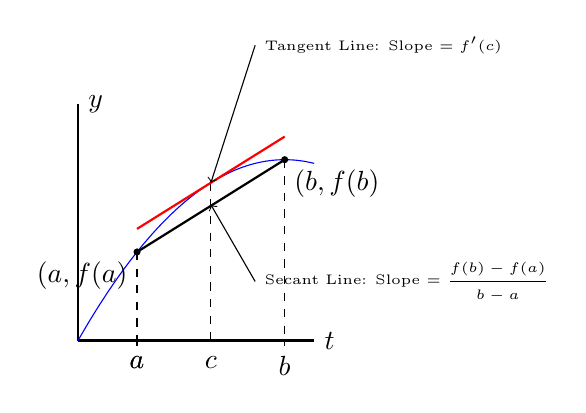
\begin{tikzpicture}[xscale=0.75,yscale=0.75]
        \draw[-,thick] (0,0) -- (4,0) node[right] {$t$};
         \draw[-,thick] (0,0) -- (0,4) node[right] {$y$};
         \draw (1,0.1) -- (1, -0.1) node[below] {$a$};
            \draw[-,dashed] (1,1.5) -- (1, -0.1) node[below] {$a$};
              \draw[-,dashed] (2.25,2.67188) -- (2.25, -0.1) node[below] {$c$};
               \draw[-,dashed] (3.5,3.0625) -- (3.5, -0.1) node[below] {$b$};
	
	
	\draw[-,smooth,domain=0:4,blue] plot(\x,{-0.25*\x*(\x-7)});
	\draw[-,thick] (1,1.5) -- (3.5,3.0625);
	\draw[fill=black] (1,1.5) circle (0.05cm) node[below left] {$(a,f(a)$};
	\draw[fill=black] (3.5,3.0625) circle (0.05cm) node[below right] {$(b,f(b)$};
	\draw[-,smooth,domain=1:3.5,red,thick] plot(\x,{0.625*\x+1.26563});
	
	
	\draw[<-,thin] (2.25,2.67) -- (3,5) node[right]{\tiny{Tangent Line: Slope $=f'(c)$}};
	\draw[<-,thin] (2.25,2.3) -- (3,1) node[right]{\tiny{Secant Line: Slope $=\dfrac{f(b)-f(a)}{b-a}$}};
	

\end{tikzpicture}

	
\end{document}
